\documentclass[11pt]{article}
\usepackage[margin=1in]{geometry}
\usepackage{listings,xcolor,hyperref,booktabs,longtable,tikz}
\usetikzlibrary{arrows.meta,positioning,shapes.geometric}
\lstset{basicstyle=\ttfamily\small,breaklines=true,frame=single,numbers=left,numberstyle=\tiny\color{gray}}

\definecolor{codebg}{RGB}{248,248,248}
\definecolor{codegreen}{RGB}{0,128,0}
\definecolor{codegray}{RGB}{128,128,128}
\definecolor{codeblue}{RGB}{0,0,180}
\definecolor{codepurple}{RGB}{128,0,128}

\lstdefinelanguage{TypeScript}{
  keywords={export,type,interface,const,class,function,async,await,import,from,
            new,return,switch,case,default,if,break,for,of,let,private,readonly,
            extends,implements,throws,try,catch,finally,true,false,undefined,null,
            this,void,Promise,Record,string,number,boolean,unknown,any},
  keywordstyle=\color{codeblue}\bfseries,
  sensitive=true,
  comment=[l]{//},
  morecomment=[s]{/*}{*/},
  commentstyle=\color{codegreen}\itshape,
  stringstyle=\color{codepurple},
  morestring=[b]',
  morestring=[b]",
  morestring=[b]`,
  backgroundcolor=\color{codebg},
}

\lstdefinelanguage{Python}{
  keywords={class,def,return,if,elif,else,for,in,import,from,async,await,
            True,False,None,self,try,except,finally,with,as,yield,not,and,or,
            Optional,Dict,List,Tuple,Any,str,int,float,bool},
  keywordstyle=\color{codeblue}\bfseries,
  sensitive=true,
  comment=[l]{\#},
  morecomment=[s]{"""}{"""},
  commentstyle=\color{codegreen}\itshape,
  stringstyle=\color{codepurple},
  morestring=[b]',
  morestring=[b]",
  backgroundcolor=\color{codebg},
}

\lstdefinelanguage{CDS}{
  keywords={service,action,type,returns,array,of,not,null,default,
            String,Integer,Double,Boolean},
  keywordstyle=\color{codeblue}\bfseries,
  sensitive=true,
  comment=[l]{//},
  morecomment=[s]{/*}{*/},
  commentstyle=\color{codegreen}\itshape,
  stringstyle=\color{codepurple},
  morestring=[b]',
  morestring=[b]",
  backgroundcolor=\color{codebg},
}

\title{Prompt-to-Response Routing:\\Multi-Layer Intelligent Request Classification}
\author{SAP OSS Technical Documentation}
\date{March 2026}

\begin{document}
\maketitle

\begin{abstract}
This document provides a comprehensive technical analysis of the prompt-to-response
routing system implemented across the SAP OSS service mesh. The system employs a
multi-layer classification architecture spanning three runtimes---a TypeScript
\texttt{IntentRouter} within the CAP LLM Plugin, a Python \texttt{MeshRouter}
in the AI Core Streaming service, and a FastAPI OpenAI-compatible gateway---to
enforce governance, security classification, and intelligent backend selection
for every LLM request. We present the cascading decision tree, security routing
maps, keyword-based content analysis, schema generation with component deny lists,
CDS service contracts, and the SSE streaming protocol, with exact code evidence
from the source files.
\end{abstract}

\tableofcontents
\newpage

% ═══════════════════════════════════════════════════════════════════════════════
\section{IntentRouter: TypeScript Cascading Decision Tree}
\label{sec:intent-router}
% ═══════════════════════════════════════════════════════════════════════════════

\noindent\textbf{Source:}
\texttt{src/data/cap-llm-plugin-main/srv/ag-ui/intent-router.ts}

The \texttt{IntentRouter} class is the TypeScript-side routing engine that runs
within the CAP LLM Plugin Node.js process. It implements a strict seven-level
cascading priority scheme, documented in the file header (lines~3--14):

\begin{lstlisting}[language=TypeScript,caption={Priority order comment (intent-router.ts, lines 3--14)},firstnumber=3]
/**
 * IntentRouter -- TypeScript port of
 *    ai-core-streaming/openai/router.py MeshRouter.
 *
 * Priority order:
 *   1. Forced header (X-Mesh-Force)
 *   2. Service-ID policy map
 *   3. Security class
 *   4. Model alias (confidential -> local model)
 *   5. Model name -> backend map
 *   6. Content keyword analysis
 *   7. Default -> aicore-streaming
 */
\end{lstlisting}

\subsection{Route Types and Decision Structure}

The router defines five possible backend targets and returns a typed
\texttt{RouteDecision} struct (lines~20--26):

\begin{lstlisting}[language=TypeScript,caption={RouteBackend and RouteDecision (intent-router.ts, lines 20--26)},firstnumber=20]
export type RouteBackend =
  'blocked' | 'vllm' | 'pal' | 'rag' | 'aicore-streaming';

export interface RouteDecision {
  backend: RouteBackend;
  reason: string;
  endpoint?: string;
}
\end{lstlisting}

\subsection{SERVICE\_ROUTING Map (7 Services)}

The \texttt{SERVICE\_ROUTING} constant maps service identifiers to backend
targets. This is the second-highest priority after forced headers
(lines~85--94):

\begin{lstlisting}[language=TypeScript,caption={SERVICE\_ROUTING map (intent-router.ts, lines 85--94)},firstnumber=85]
const SERVICE_ROUTING: Record<string, RouteBackend> = {
  'data-cleaning-copilot': 'vllm',
  'gen-ai-toolkit-hana': 'vllm',
  'ai-core-pal': 'pal',
  'langchain-hana': 'vllm',
  'odata-vocabularies': 'aicore-streaming',
  'ui5-webcomponents-ngx': 'aicore-streaming',
  'world-monitor': 'aicore-streaming',
};
\end{lstlisting}

\begin{table}[h]
\centering
\caption{SERVICE\_ROUTING: Service-ID to Backend Mapping}
\begin{tabular}{@{}ll@{}}
\toprule
\textbf{Service ID} & \textbf{Backend} \\
\midrule
\texttt{data-cleaning-copilot} & \texttt{vllm} \\
\texttt{gen-ai-toolkit-hana} & \texttt{vllm} \\
\texttt{ai-core-pal} & \texttt{pal} \\
\texttt{langchain-hana} & \texttt{vllm} \\
\texttt{odata-vocabularies} & \texttt{aicore-streaming} \\
\texttt{ui5-webcomponents-ngx} & \texttt{aicore-streaming} \\
\texttt{world-monitor} & \texttt{aicore-streaming} \\
\bottomrule
\end{tabular}
\end{table}

\subsection{SECURITY\_ROUTING Map (4 Classes)}

Security classification is the third priority level. Four classes map to three
distinct behaviors (lines~97--102):

\begin{lstlisting}[language=TypeScript,caption={SECURITY\_ROUTING map (intent-router.ts, lines 97--102)},firstnumber=97]
const SECURITY_ROUTING: Record<string, RouteBackend> = {
  public: 'aicore-streaming',
  internal: 'aicore-streaming',
  confidential: 'vllm',
  restricted: 'blocked',
};
\end{lstlisting}

\begin{table}[h]
\centering
\caption{SECURITY\_ROUTING: Security Classification to Backend Mapping}
\begin{tabular}{@{}lll@{}}
\toprule
\textbf{Security Class} & \textbf{Backend} & \textbf{Behavior} \\
\midrule
\texttt{public} & \texttt{aicore-streaming} & SAP AI Core (cloud) \\
\texttt{internal} & \texttt{aicore-streaming} & SAP AI Core (cloud) \\
\texttt{confidential} & \texttt{vllm} & On-premise vLLM (Qwen3.5) \\
\texttt{restricted} & \texttt{blocked} & Request rejected (HTTP 403) \\
\bottomrule
\end{tabular}
\end{table}

\subsection{MODEL\_ALIASES: Confidential Qwen3.5 Variants}

When a caller specifies a confidential model alias, the router transparently
redirects to the corresponding on-premise Qwen3.5 model (lines~116--120):

\begin{lstlisting}[language=TypeScript,caption={MODEL\_ALIASES (intent-router.ts, lines 116--120)},firstnumber=116]
const MODEL_ALIASES: Record<string, string> = {
  'qwen3.5-confidential': 'Qwen/Qwen3.5-35B',
  'qwen3.5-0.8b-confidential': 'Qwen/Qwen3.5-0.8B',
  'qwen3.5-9b-confidential': 'Qwen/Qwen3.5-9B',
};
\end{lstlisting}

The full model-to-backend map additionally covers the non-aliased Qwen3.5
family with both HuggingFace-style and short-form identifiers (lines~105--113):

\begin{lstlisting}[language=TypeScript,caption={MODEL\_BACKEND map (intent-router.ts, lines 105--113)},firstnumber=105]
const MODEL_BACKEND: Record<string, RouteBackend> = {
  'Qwen/Qwen3.5-0.8B': 'vllm',
  'Qwen/Qwen3.5-9B': 'vllm',
  'Qwen/Qwen3.5-35B': 'vllm',
  // Short aliases
  'qwen3.5-0.8b': 'vllm',
  'qwen3.5-9b': 'vllm',
  'qwen3.5-35b': 'vllm',
};
\end{lstlisting}

\subsection{Content Keyword Analysis}

At priority level 6, the router inspects the lowercased message content for
three keyword categories. This is the last classification step before the
default fallback.

\subsubsection{CONFIDENTIAL\_KEYWORDS}

These keywords trigger routing to the on-premise vLLM backend
(lines~127--136):

\begin{lstlisting}[language=TypeScript,caption={DEFAULT\_CONFIDENTIAL\_KEYWORDS (intent-router.ts, lines 127--136)},firstnumber=127]
const DEFAULT_CONFIDENTIAL_KEYWORDS: string[] = [
  // Business entities
  'customer', 'order', 'invoice', 'contract', 'supplier',
  'business partner', 'cds entity', 'cap service',
  // Financial
  'revenue', 'profit', 'cost', 'budget', 'forecast',
  // Personal / credential
  'personal', 'private', 'confidential',
  'salary', 'ssn', 'credit_card', 'password',
];
\end{lstlisting}

\subsubsection{RESTRICTED\_KEYWORDS}

These keywords cause the request to be blocked entirely (lines~142--144):

\begin{lstlisting}[language=TypeScript,caption={RESTRICTED\_KEYWORDS (intent-router.ts, lines 142--144)},firstnumber=142]
const RESTRICTED_KEYWORDS: string[] = [
  'restricted', 'classified', 'secret',
];
\end{lstlisting}

\subsubsection{PAL\_KEYWORDS}

These keywords route the request to the SAP HANA PAL analytics backend
(lines~147--151):

\begin{lstlisting}[language=TypeScript,caption={DEFAULT\_PAL\_KEYWORDS (intent-router.ts, lines 147--151)},firstnumber=147]
const DEFAULT_PAL_KEYWORDS: string[] = [
  'forecast', 'predict', 'regression', 'classification',
  'cluster', 'clustering',
  'anomaly', 'detect', 'arima', 'kmeans', 'k-means',
  'segment', 'segmentation',
  'time series', 'timeseries', 'outlier',
  'pal algorithm', 'hana pal',
];
\end{lstlisting}

\subsection{The classify() Method}

The core routing logic is implemented in the \texttt{classify()} method
(lines~178--282). The method accepts a message string and an options object
containing optional routing hints, and returns a \texttt{RouteDecision}:

\begin{lstlisting}[language=TypeScript,caption={classify() method signature (intent-router.ts, lines 178--187)},firstnumber=178]
classify(
  message: string,
  options: {
    model?: string;
    serviceId?: string;
    securityClass?: string;
    forceBackend?: RouteBackend;
    enableRag?: boolean;
  } = {}
): RouteDecision {
\end{lstlisting}

The cascading decision steps within \texttt{classify()} are:

\begin{enumerate}
  \item \textbf{Forced backend} (line~192): If \texttt{forceBackend} is set,
        return immediately with that backend.
  \item \textbf{Service-ID policy} (line~204): Look up \texttt{serviceId} in
        \texttt{SERVICE\_ROUTING}.
  \item \textbf{Security class} (line~214): Look up \texttt{securityClass} in
        \texttt{SECURITY\_ROUTING}; \texttt{restricted} returns \texttt{blocked}.
  \item \textbf{Model alias} (line~227): Check \texttt{MODEL\_ALIASES} for
        confidential model redirection.
  \item \textbf{Model name} (line~236): Check \texttt{MODEL\_BACKEND} for
        direct model-to-backend mapping.
  \item \textbf{Content keywords} (lines~246--274):
    \begin{enumerate}
      \item Restricted keywords (line~246) $\rightarrow$ \texttt{blocked}
      \item Confidential keywords (line~251) $\rightarrow$ \texttt{vllm}
      \item PAL keywords (line~260) $\rightarrow$ \texttt{pal}
      \item RAG enabled (line~269) $\rightarrow$ \texttt{rag}
    \end{enumerate}
  \item \textbf{Default} (line~277): Fall through to \texttt{aicore-streaming}.
\end{enumerate}

\begin{figure}[h]
\centering
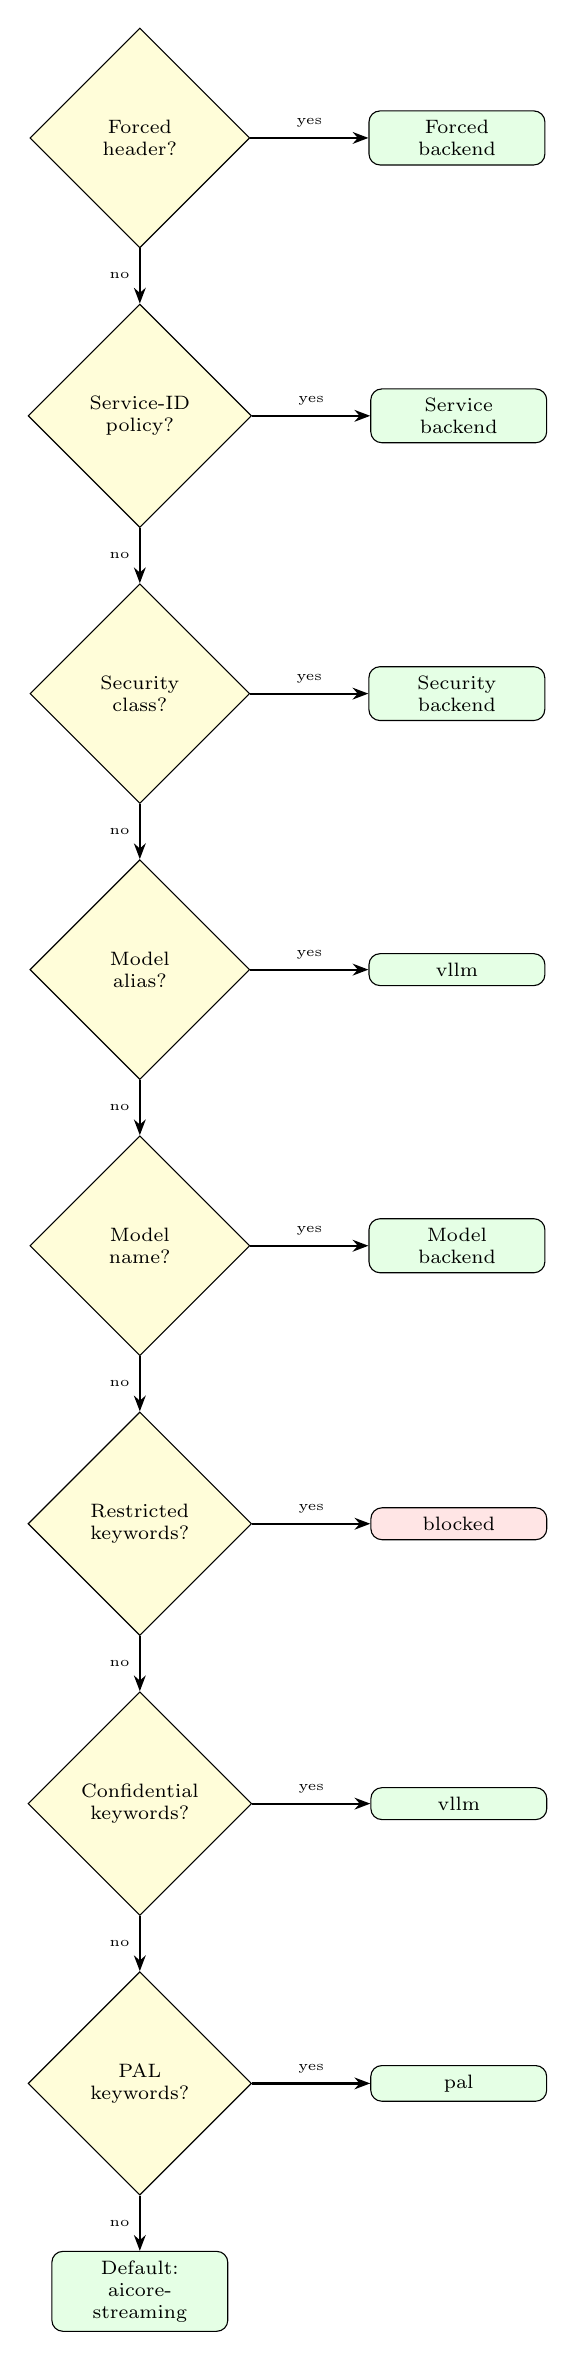
\begin{tikzpicture}[
  node distance=0.7cm and 1.5cm,
  decision/.style={diamond, draw, fill=yellow!15, text width=2.2cm,
                   align=center, inner sep=1pt, font=\scriptsize},
  result/.style={rectangle, rounded corners, draw, fill=green!10,
                 text width=2cm, align=center, font=\scriptsize},
  block/.style={rectangle, rounded corners, draw, fill=red!10,
                text width=2cm, align=center, font=\scriptsize},
  arr/.style={-{Stealth[length=2mm]}, thick},
]
  \node[decision] (d1) {Forced\\header?};
  \node[decision, below=of d1] (d2) {Service-ID\\policy?};
  \node[decision, below=of d2] (d3) {Security\\class?};
  \node[decision, below=of d3] (d4) {Model\\alias?};
  \node[decision, below=of d4] (d5) {Model\\name?};
  \node[decision, below=of d5] (d6) {Restricted\\keywords?};
  \node[decision, below=of d6] (d7) {Confidential\\keywords?};
  \node[decision, below=of d7] (d8) {PAL\\keywords?};
  \node[result, below=of d8] (def) {Default:\\aicore-\\streaming};

  \node[result, right=of d1] (r1) {Forced\\backend};
  \node[result, right=of d2] (r2) {Service\\backend};
  \node[result, right=of d3] (r3) {Security\\backend};
  \node[result, right=of d4] (r4) {vllm};
  \node[result, right=of d5] (r5) {Model\\backend};
  \node[block, right=of d6] (r6) {blocked};
  \node[result, right=of d7] (r7) {vllm};
  \node[result, right=of d8] (r8) {pal};

  \draw[arr] (d1) -- node[left,font=\tiny]{no} (d2);
  \draw[arr] (d2) -- node[left,font=\tiny]{no} (d3);
  \draw[arr] (d3) -- node[left,font=\tiny]{no} (d4);
  \draw[arr] (d4) -- node[left,font=\tiny]{no} (d5);
  \draw[arr] (d5) -- node[left,font=\tiny]{no} (d6);
  \draw[arr] (d6) -- node[left,font=\tiny]{no} (d7);
  \draw[arr] (d7) -- node[left,font=\tiny]{no} (d8);
  \draw[arr] (d8) -- node[left,font=\tiny]{no} (def);

  \draw[arr] (d1) -- node[above,font=\tiny]{yes} (r1);
  \draw[arr] (d2) -- node[above,font=\tiny]{yes} (r2);
  \draw[arr] (d3) -- node[above,font=\tiny]{yes} (r3);
  \draw[arr] (d4) -- node[above,font=\tiny]{yes} (r4);
  \draw[arr] (d5) -- node[above,font=\tiny]{yes} (r5);
  \draw[arr] (d6) -- node[above,font=\tiny]{yes} (r6);
  \draw[arr] (d7) -- node[above,font=\tiny]{yes} (r7);
  \draw[arr] (d8) -- node[above,font=\tiny]{yes} (r8);
\end{tikzpicture}
\caption{IntentRouter cascading decision tree}
\label{fig:decision-tree}
\end{figure}

% ═══════════════════════════════════════════════════════════════════════════════
\section{AG-UI Agent Service: Request Handling and SSE Emission}
\label{sec:agent-service}
% ═══════════════════════════════════════════════════════════════════════════════

\noindent\textbf{Source:}
\texttt{src/data/cap-llm-plugin-main/srv/ag-ui/agent-service.ts}

The \texttt{AgUiAgentService} class is the main orchestrator for the AG-UI
protocol. It coordinates incoming requests, emits AG-UI events via
Server-Sent Events (SSE), and delegates to specialized backend handlers based
on the \texttt{IntentRouter} decision.

\subsection{Route Backends and Behavior}

The file header documents the five backend behaviors (lines~9--14):

\begin{lstlisting}[language=TypeScript,caption={Route backend documentation (agent-service.ts, lines 9--14)},firstnumber=9]
 *   blocked          -> 403, no LLM call
 *   vllm             -> @sap-ai-sdk/vllm VllmChatClient
 *   pal              -> PalClient -> ai-core-pal MCP :8084
 *   rag              -> HANAVectorStore + OrchestrationClient
 *   aicore-streaming -> ai-core-streaming MCP :9190
\end{lstlisting}

\subsection{handleRunRequest Method}

The \texttt{handleRunRequest} method (lines~130--244) is the entry point for
all AG-UI run requests. It follows this sequence:

\begin{enumerate}
  \item Set SSE headers (\texttt{text/event-stream}, \texttt{no-cache},
        \texttt{keep-alive}) on lines~135--139.
  \item Create or retrieve a session (lines~142--148).
  \item Extract the user message (line~154).
  \item Invoke the \texttt{IntentRouter.classify()} method (lines~158--164).
  \item Handle the \texttt{blocked} case with HTTP 403 (lines~171--181).
  \item Emit \texttt{RUN\_STARTED} event (line~184).
  \item Dispatch to backend-specific handler via \texttt{switch} (lines~197--212).
  \item Emit the final \texttt{UI\_SCHEMA\_SNAPSHOT} and \texttt{RUN\_FINISHED} events
        (lines~217--224).
\end{enumerate}

\begin{lstlisting}[language=TypeScript,caption={Routing decision and dispatch (agent-service.ts, lines 156--212)},firstnumber=156]
    // Routing decision
    const forceBackend = (request as any).forceBackend;
    const route: RouteDecision =
      this.intentRouter.classify(userMessage, {
        model: this.config.chatModelName,
        serviceId: this.config.serviceId,
        securityClass: this.config.securityClass,
        forceBackend,
        enableRag: this.config.enableRag
                   && !!this.config.ragTable,
      });

    LOG.info(`AG-UI routing decision: `
      + `${route.backend} -- ${route.reason}`);

    // Blocked -- emit error and exit
    if (route.backend === 'blocked') {
      httpRes.statusCode = 403;
      this.writeEvent(httpRes,
        AgUiEventType.RUN_ERROR, {
          runId,
          message: `Request blocked: ${route.reason}`,
          code: 'REQUEST_BLOCKED',
        });
      httpRes.write(
        createErrorFrame('REQUEST_BLOCKED', route.reason));
      httpRes.end();
      return;
    }

    // ... [RUN_STARTED, loading UI, STEP_STARTED] ...

    switch (route.backend) {
      case 'vllm':
        schema = await this.generateSchemaViaVllm(
          userMessage, session, httpRes, runId, threadId);
        break;
      case 'pal':
        schema = await this.generateSchemaViaPal(
          userMessage, session, httpRes, runId, threadId);
        break;
      case 'rag':
        schema = await this.generateSchemaWithRag(
          userMessage, session, httpRes, runId, threadId);
        break;
      case 'aicore-streaming':
        schema = await this.generateSchemaViaAicoreStreaming(
          userMessage, session, httpRes, runId, threadId);
        break;
      default:
        schema = await this.generateSchemaDirectly(
          userMessage, session);
    }
\end{lstlisting}

\subsection{Backend Handler Details}

\begin{description}
  \item[\texttt{vllm} (lines 310--372):] Uses \texttt{@sap-ai-sdk/vllm
        VllmChatClient} when available, falls back to raw HTTP against the
        vLLM OpenAI-compatible endpoint (\texttt{/v1/chat/completions}).
        Default model: \texttt{Qwen/Qwen3.5-35B}.

  \item[\texttt{pal} (lines 378--390):] Delegates to \texttt{PalClient} which
        calls the \texttt{ai-core-pal} MCP server on port 8084.

  \item[\texttt{rag} (lines 396--430):] Embeds the user message via the LLM
        plugin, performs similarity search against
        \texttt{HANAVectorStore} using \texttt{COSINE\_SIMILARITY}, retrieves
        top-3 documents, then passes the context-augmented prompt to the
        \texttt{SchemaGenerator}.

  \item[\texttt{aicore-streaming} (lines 437--511):] Uses
        \texttt{@sap-ai-sdk/mcp-server AISdkMcpClient} when available, falls
        back to raw MCP JSON-RPC to the \texttt{stream\_complete} tool on port
        9190.
\end{description}

% ═══════════════════════════════════════════════════════════════════════════════
\section{Python MeshRouter: Smart Router with Governance Rules}
\label{sec:mesh-router}
% ═══════════════════════════════════════════════════════════════════════════════

\noindent\textbf{Source:}
\texttt{src/data/ai-core-streaming/openai/router.py}

The Python \texttt{MeshRouter} class mirrors the TypeScript \texttt{IntentRouter}
and runs within the FastAPI server process. It provides the same cascading
priority scheme but with Python-native data structures and an integrated
audit log.

\subsection{BACKENDS Configuration}

The router defines two backend endpoints configurable via environment variables
(lines~23--26):

\begin{lstlisting}[language=Python,caption={BACKENDS config (router.py, lines 23--26)},firstnumber=23]
BACKENDS = {
    "ai-core-streaming": os.environ.get(
        "AICORE_STREAMING_URL",
        "http://localhost:9190/v1"),
    "vllm": os.environ.get(
        "VLLM_URL", "http://localhost:9180/v1"),
}
\end{lstlisting}

\subsection{Security and Service Routing}

The Python router's security class mapping differs slightly from the TypeScript
version---\texttt{restricted} maps to \texttt{vllm} rather than \texttt{blocked}
(lines~29--34):

\begin{lstlisting}[language=Python,caption={SECURITY\_ROUTING (router.py, lines 29--34)},firstnumber=29]
SECURITY_ROUTING = {
    "public": "ai-core-streaming",
    "internal": "ai-core-streaming",
    "confidential": "vllm",
    "restricted": "vllm"
}
\end{lstlisting}

The service routing map covers 7 services (lines~37--45):

\begin{lstlisting}[language=Python,caption={SERVICE\_ROUTING (router.py, lines 37--45)},firstnumber=37]
SERVICE_ROUTING = {
    "data-cleaning-copilot": "vllm",
    "gen-ai-toolkit-hana": "vllm",
    "ai-core-pal": "vllm",
    "langchain-hana": "vllm",
    "odata-vocabularies": "ai-core-streaming",
    "ui5-webcomponents-ngx": "ai-core-streaming",
    "world-monitor": "ai-core-streaming",
}
\end{lstlisting}

\subsection{Content Analysis}

The Python router extracts content from chat messages, prompt text, and
embedding inputs (lines~172--195):

\begin{lstlisting}[language=Python,caption={Content extraction (router.py, lines 172--195)},firstnumber=172]
def _extract_content(self, request: Dict[str, Any])
    -> str:
    """Extract text content from request."""
    content_parts = []

    # Chat completions
    messages = request.get("messages", [])
    for msg in messages:
        if isinstance(msg, dict) and "content" in msg:
            content_parts.append(str(msg["content"]))

    # Completions
    prompt = request.get("prompt", "")
    if prompt:
        content_parts.append(str(prompt))

    # Embeddings
    input_text = request.get("input", "")
    if input_text:
        if isinstance(input_text, list):
            content_parts.extend(
                [str(t) for t in input_text])
        else:
            content_parts.append(str(input_text))

    return " ".join(content_parts).lower()
\end{lstlisting}

\subsection{Audit Logging}

The \texttt{log\_routing} method records every routing decision with a
structured audit entry containing six fields (lines~238--258):

\begin{lstlisting}[language=Python,caption={Audit logging (router.py, lines 238--258)},firstnumber=238]
def log_routing(
    self,
    request_id: str,
    backend: str,
    reason: str,
    model: str,
    status: str,
    trace_id: Optional[str] = None
):
    """Log routing decision for audit."""
    entry = {
        "timestamp": datetime.now(
            timezone.utc).isoformat(),
        "request_id": request_id,
        "backend": backend,
        "reason": reason,
        "model": model,
        "status": status,
    }
    if trace_id:
        entry["trace_id"] = trace_id
    self.audit_log.append(entry)
\end{lstlisting}

\begin{table}[h]
\centering
\caption{Audit Log Entry Fields}
\begin{tabular}{@{}lll@{}}
\toprule
\textbf{Field} & \textbf{Type} & \textbf{Description} \\
\midrule
\texttt{timestamp} & ISO 8601 & UTC timestamp of routing decision \\
\texttt{request\_id} & string & Unique identifier for the request \\
\texttt{backend} & string & Selected backend (\texttt{ai-core-streaming} or \texttt{vllm}) \\
\texttt{reason} & string & Human-readable routing reason \\
\texttt{model} & string & Requested model name \\
\texttt{status} & string & Request status (e.g., \texttt{streaming}) \\
\texttt{trace\_id} & string? & W3C trace ID or correlation ID \\
\bottomrule
\end{tabular}
\end{table}

% ═══════════════════════════════════════════════════════════════════════════════
\section{FastAPI OpenAI-Compatible Server}
\label{sec:server}
% ═══════════════════════════════════════════════════════════════════════════════

\noindent\textbf{Source:}
\texttt{src/data/ai-core-streaming/openai/server.py}

The FastAPI server exposes an OpenAI-compatible API surface with integrated
governance routing. It is deployed as a KServe InferenceService on SAP AI Core.

\subsection{Health Endpoints}

Four health check endpoints are registered for KServe compatibility
(lines~129--141):

\begin{lstlisting}[language=Python,caption={Health endpoints (server.py, lines 129--141)},firstnumber=129]
@app.get("/health")
@app.get("/healthz")
@app.get("/ready")
@app.get("/readyz")
async def health():
    """Health check endpoint for KServe."""
    return {"status": "healthy",
            "timestamp": time.time()}

@app.get("/v1/health")
async def health_v1():
    """Health check under v1 prefix."""
    return {"status": "healthy",
            "timestamp": time.time()}
\end{lstlisting}

\subsection{POST /v1/chat/completions}

The chat completions endpoint accepts governance headers for routing control
(lines~186--227):

\begin{lstlisting}[language=Python,caption={Chat completions endpoint with governance headers (server.py, lines 186--194)},firstnumber=186]
@app.post("/v1/chat/completions")
async def chat_completions(
    request: ChatCompletionRequest,
    x_mesh_service: Optional[str] =
        Header(None, alias="X-Mesh-Service"),
    x_mesh_security_class: Optional[str] =
        Header(None, alias="X-Mesh-Security-Class"),
    x_mesh_routing: Optional[str] =
        Header(None, alias="X-Mesh-Routing"),
    traceparent: Optional[str] = Header(None),
    x_correlation_id: Optional[str] =
        Header(None, alias="X-Correlation-ID"),
):
\end{lstlisting}

\begin{table}[h]
\centering
\caption{Governance Headers for Routing Control}
\begin{tabular}{@{}lll@{}}
\toprule
\textbf{Header} & \textbf{Purpose} & \textbf{Router Input} \\
\midrule
\texttt{X-Mesh-Service} & Service identifier & \texttt{service\_id} \\
\texttt{X-Mesh-Security-Class} & Security classification & \texttt{security\_class} \\
\texttt{X-Mesh-Routing} & Force specific backend & \texttt{force\_backend} \\
\texttt{traceparent} & W3C distributed tracing & \texttt{trace\_id} \\
\texttt{X-Correlation-ID} & Fallback correlation & \texttt{trace\_id} \\
\bottomrule
\end{tabular}
\end{table}

\subsection{Streaming SSE Support}

When \texttt{stream=true}, the endpoint returns a \texttt{StreamingResponse}
with SSE frames. The streaming generator emits delta chunks and a final
\texttt{[DONE]} sentinel (lines~230--277):

\begin{lstlisting}[language=Python,caption={SSE streaming generator (server.py, lines 230--277)},firstnumber=230]
async def stream_chat_completion(
    request: Dict, headers: Dict,
    trace_id: Optional[str] = None):
    """Generate SSE stream for chat completion."""
    request_id = f"chatcmpl-{uuid.uuid4().hex[:24]}"
    model = request.get("model", "gpt-4")

    # Route to determine backend
    backend, endpoint, reason = router.route(
        request,
        service_id=headers.get("X-Mesh-Service"),
        security_class=headers.get(
            "X-Mesh-Security-Class"),
        force_backend=headers.get("X-Mesh-Routing"),
        trace_id=trace_id,
    )
    router.log_routing(request_id, backend, reason,
                       model, "streaming",
                       trace_id=trace_id)

    # ... [delta chunk emission] ...

    # Final chunk
    final_chunk = { ... "finish_reason": "stop" ... }
    yield f"data: {json.dumps(final_chunk)}\n\n"
    yield "data: [DONE]\n\n"
\end{lstlisting}

\subsection{Additional Endpoints}

\begin{description}
  \item[\texttt{POST /v1/embeddings} (lines 361--390):] OpenAI-compatible
        embedding generation with the same three governance headers.
  \item[\texttt{GET /v1/models} (lines 145--162):] Lists available models
        across both AI Core and vLLM backends (10 models total).
  \item[\texttt{GET /v1/routing/info} (lines 394--402):] SAP extension
        returning the complete routing configuration (backends, security
        routing, model backend, service routing).
  \item[\texttt{GET /v1/routing/audit} (lines 405--410):] SAP extension
        returning the full routing audit log.
\end{description}

% ═══════════════════════════════════════════════════════════════════════════════
\section{CAP LLM Plugin Routing}
\label{sec:cap-llm-plugin}
% ═══════════════════════════════════════════════════════════════════════════════

\noindent\textbf{Source:}
\texttt{src/data/cap-llm-plugin-main/srv/cap-llm-plugin.ts}

The \texttt{CAPLLMPlugin} class extends \texttt{cds.Service} and implements
the core LLM operations. It integrates the \texttt{@sap-ai-sdk/orchestration}
SDK for chat completions, embeddings, and content safety filtering.

\subsection{getChatCompletionWithConfig}

This method (lines~315--386) creates an \texttt{OrchestrationClient} with
prompt templating and executes chat completion. It logs token usage via
OpenTelemetry spans:

\begin{lstlisting}[language=TypeScript,caption={getChatCompletionWithConfig with token logging (cap-llm-plugin.ts, lines 315--365)},firstnumber=315]
async getChatCompletionWithConfig(
    config: ChatConfig,
    payload: unknown): Promise<unknown> {
  const span = getTracer().startSpan(
    "cap-llm-plugin.getChatCompletionWithConfig");

  // ... [config validation] ...

  const { OrchestrationClient } =
    await import("@sap-ai-sdk/orchestration");

  const client = new OrchestrationClient({
    promptTemplating: {
      model: { name: config.modelName as any },
    },
  }, { resourceGroup: config.resourceGroup });

  const response = await client.chatCompletion(
    { messages }, { middleware: [
      createOtelMiddleware({ ... }),
    ]});

  // Log token usage for cost/quality observability
  const usage =
    (response as any)?.getTokenUsage?.();
  if (usage) {
    span.setAttribute(
      "llm.usage.prompt_tokens",
      usage.prompt_tokens ?? 0);
    span.setAttribute(
      "llm.usage.completion_tokens",
      usage.completion_tokens ?? 0);
    span.setAttribute(
      "llm.usage.total_tokens",
      usage.total_tokens ?? 0);
  }

  return response;
}
\end{lstlisting}

\subsection{getHarmonizedChatCompletion}

This method (lines~790--845) provides chat completion with response extraction
flags. Only the first truthy flag takes effect (lines~823--832):

\begin{lstlisting}[language=TypeScript,caption={Response extraction flags (cap-llm-plugin.ts, lines 823--832)},firstnumber=823]
switch (true) {
  case getContent:
    return response.getContent();
  case getTokenUsage:
    return response.getTokenUsage();
  case getFinishReason:
    return response.getFinishReason();
  default:
    return response;
}
\end{lstlisting}

\subsection{streamChatCompletion}

The streaming method (lines~869--982) writes SSE frames directly to the HTTP
response. The frame protocol consists of four message types:

\begin{lstlisting}[language=TypeScript,caption={SSE frame emission (cap-llm-plugin.ts, lines 931--949)},firstnumber=931]
if (isStreaming) {
  const frame = JSON.stringify(
    { delta, index: 0 });
  httpRes!.write(`data: ${frame}\n\n`);
}

// ... after stream completes ...

if (isStreaming) {
  const doneFrame = JSON.stringify(
    { finishReason, totalTokens });
  httpRes!.write(`data: ${doneFrame}\n\n`);
  httpRes!.write("data: [DONE]\n\n");
  httpRes!.end();
  return "";
}
\end{lstlisting}

Error frames use a distinct SSE event type (lines~962--964):

\begin{lstlisting}[language=TypeScript,caption={Error frame emission (cap-llm-plugin.ts, lines 962--964)},firstnumber=962]
const errFrame = JSON.stringify(
  { code: "CHAT_STREAM_FAILED",
    message: err.message });
httpRes!.write(
  `event: error\ndata: ${errFrame}\n\n`);
\end{lstlisting}

\begin{table}[h]
\centering
\caption{SSE Frame Protocol for streamChatCompletion}
\begin{tabular}{@{}lll@{}}
\toprule
\textbf{Frame Type} & \textbf{SSE Format} & \textbf{Example} \\
\midrule
Delta & \texttt{data: \{"delta":"...","index":0\}} & Token-by-token content \\
Done & \texttt{data: \{"finishReason":"stop","totalTokens":42\}} & Completion metadata \\
Sentinel & \texttt{data: [DONE]} & End-of-stream marker \\
Error & \texttt{event: error\textbackslash ndata: \{"code":"...","message":"..."\}} & Error notification \\
\bottomrule
\end{tabular}
\end{table}

\subsection{getContentFilters}

The content filter method (lines~1003--1038) currently supports only Azure
Content Safety filters. It uses the \texttt{buildAzureContentSafetyFilter}
function from the SAP AI SDK:

\begin{lstlisting}[language=TypeScript,caption={getContentFilters (cap-llm-plugin.ts, lines 1003--1022)},firstnumber=1003]
async getContentFilters(
    { type, config }: ContentFilterParams)
    : Promise<unknown> {
  if (type.toLowerCase() !== "azure") {
    throw new ChatCompletionError(
      `Unsupported type ${type}. `
      + `Currently supported: 'azure'.`,
      "UNSUPPORTED_FILTER_TYPE",
      { type, supportedTypes: ["azure"] });
  }

  const { buildAzureContentSafetyFilter } =
    await import("@sap-ai-sdk/orchestration");
  const result =
    buildAzureContentSafetyFilter(config as any);
  return result;
}
\end{lstlisting}

% ═══════════════════════════════════════════════════════════════════════════════
\section{Schema Generator: Component Whitelist and Deny List}
\label{sec:schema-generator}
% ═══════════════════════════════════════════════════════════════════════════════

\noindent\textbf{Source:}
\texttt{src/data/cap-llm-plugin-main/srv/ag-ui/schema-generator.ts}

The \texttt{SchemaGenerator} class uses LLM function calling to generate
\texttt{A2UiSchema} structures from natural language. It enforces a strict
security model through component whitelisting and deny listing.

\subsection{SCHEMA\_GEN\_DENY\_LIST}

Four components are explicitly blocked for security reasons (lines~22--27):

\begin{lstlisting}[language=TypeScript,caption={SCHEMA\_GEN\_DENY\_LIST (schema-generator.ts, lines 22--27)},firstnumber=22]
export const SCHEMA_GEN_DENY_LIST = new Set([
  'ui5-file-uploader',
    // OS file-picker -> potential data exfiltration
  'ui5-file-chooser',
    // same risk as ui5-file-uploader
  'ui5-upload-collection',
    // agent-driven upload flows
  'ui5-upload-collection-item',
    // child of upload-collection
]);
\end{lstlisting}

\subsection{ALLOWED\_COMPONENTS Whitelist}

The whitelist contains 90+ UI5 Web Components organized into eight categories
(lines~35--89):

\begin{longtable}{@{}ll@{}}
\caption{ALLOWED\_COMPONENTS Categories (schema-generator.ts, lines 35--89)} \\
\toprule
\textbf{Category} & \textbf{Example Components} \\
\midrule
\endfirsthead
\toprule
\textbf{Category} & \textbf{Example Components} \\
\midrule
\endhead
Basic / Display & \texttt{ui5-button}, \texttt{ui5-label}, \texttt{ui5-badge}, \texttt{ui5-avatar} \\
Form components & \texttt{ui5-input}, \texttt{ui5-select}, \texttt{ui5-checkbox}, \texttt{ui5-slider} \\
Layout & \texttt{ui5-card}, \texttt{ui5-panel}, \texttt{ui5-toolbar}, \texttt{ui5-dynamic-page} \\
Data Display & \texttt{ui5-table}, \texttt{ui5-list}, \texttt{ui5-tree} \\
Navigation & \texttt{ui5-tabcontainer}, \texttt{ui5-breadcrumbs}, \texttt{ui5-wizard} \\
Feedback / Dialogs & \texttt{ui5-dialog}, \texttt{ui5-message-strip}, \texttt{ui5-toast} \\
Fiori-specific & \texttt{ui5-shellbar}, \texttt{ui5-timeline}, \texttt{ui5-notification-list} \\
AI components & \texttt{ui5-ai-button}, \texttt{ui5-ai-prompt-input} \\
Charts & \texttt{ui5-micro-bar-chart}, \texttt{ui5-radial-chart} \\
\bottomrule
\end{longtable}

\subsection{GENERATE\_UI\_FUNCTION for LLM Function Calling}

The \texttt{GENERATE\_UI\_FUNCTION} constant defines an OpenAI function-calling
schema that constrains the LLM to produce valid \texttt{A2UiSchema} output.
The \texttt{type} field is restricted to the \texttt{ALLOWED\_COMPONENTS} set
(lines~98--172):

\begin{lstlisting}[language=TypeScript,caption={GENERATE\_UI\_FUNCTION definition (schema-generator.ts, lines 98--115)},firstnumber=98]
export const GENERATE_UI_FUNCTION = {
  name: 'generate_ui',
  description: `Generate a SAP Fiori UI schema
    (A2UiSchema) based on user requirements. ...`,
  parameters: {
    type: 'object',
    properties: {
      layout: {
        type: 'object',
        properties: {
          id: { type: 'string' },
          type: {
            type: 'string',
            enum: Array.from(ALLOWED_COMPONENTS),
          },
          props: {
            type: 'object',
            additionalProperties: true,
          },
          children: {
            type: 'array',
            items: { $ref: '#/properties/layout' },
          },
          // ... [slots, dataBinding] ...
        },
        required: ['id', 'type'],
      },
      // ... [dataSources, actions] ...
    },
    required: ['layout'],
  },
};
\end{lstlisting}

\subsection{Sanitization Pipeline}

The \texttt{sanitizeComponent} method (lines~413--450) enforces the component
security model in two stages:

\begin{enumerate}
  \item Check the deny list first---denied components are replaced with a
        \texttt{ui5-text} element displaying \texttt{[Denied component: ...]}
        (lines~415--420).
  \item Check the whitelist---components not in \texttt{ALLOWED\_COMPONENTS}
        are replaced with \texttt{[Blocked component: ...]} (lines~423--429).
  \item Recursively sanitize all children and slots (lines~433--441).
  \item Strip event handlers (\texttt{on*} props) and \texttt{javascript:}
        URLs from props (lines~455--473).
\end{enumerate}

% ═══════════════════════════════════════════════════════════════════════════════
\section{CDS Service Contract}
\label{sec:cds-contract}
% ═══════════════════════════════════════════════════════════════════════════════

\noindent\textbf{Source:}
\texttt{src/data/cap-llm-plugin-main/srv/llm-service.cds}

The CDS service definition provides a typed API contract for all public
operations exposed by the CAP LLM Plugin. This contract drives OpenAPI spec
generation, typed client generation, and contract drift detection in CI.

\subsection{Shared Types}

Four core types define the request/response structures (lines~17--56):

\begin{lstlisting}[language=CDS,caption={Core CDS types (llm-service.cds, lines 31--56)},firstnumber=31]
type EmbeddingConfig {
  modelName       : String not null;
  resourceGroup   : String not null;
  destinationName : String;
  deploymentUrl   : String;
}

type ChatConfig {
  modelName       : String not null;
  resourceGroup   : String not null;
  destinationName : String;
  deploymentUrl   : String;
}

type ChatMessage {
  role    : String not null;
  content : String not null;
}

type SimilaritySearchResult {
  PAGE_CONTENT : String;
  SCORE        : Double;
}
\end{lstlisting}

\subsection{Service Action Definitions}

The \texttt{CAPLLMPluginService} defines eight public actions (lines~62--147):

\begin{longtable}{@{}llp{7cm}@{}}
\caption{CDS Service Actions} \\
\toprule
\textbf{Action} & \textbf{Line} & \textbf{Description} \\
\midrule
\endfirsthead
\toprule
\textbf{Action} & \textbf{Line} & \textbf{Description} \\
\midrule
\endhead
\texttt{getEmbeddingWithConfig} & 67 & Generate vector embeddings for input text \\
\texttt{getChatCompletionWithConfig} & 75 & Chat completion via Orchestration SDK \\
\texttt{getRagResponse} & 83 & Full RAG pipeline: embed $\rightarrow$ search $\rightarrow$ complete \\
\texttt{similaritySearch} & 102 & Vector similarity search on HANA Cloud table \\
\texttt{getAnonymizedData} & 114 & Retrieve anonymized data from HANA view \\
\texttt{getHarmonizedChatCompletion} & 122 & Chat with optional response extraction flags \\
\texttt{streamChatCompletion} & 135 & Stream tokens as Server-Sent Events \\
\texttt{getContentFilters} & 142 & Build Azure Content Safety filters \\
\bottomrule
\end{longtable}

\subsection{Streaming Action Contract}

The \texttt{streamChatCompletion} action definition includes documentation of
the SSE frame protocol (lines~130--139):

\begin{lstlisting}[language=CDS,caption={streamChatCompletion contract (llm-service.cds, lines 130--139)},firstnumber=130]
/** Stream chat completion tokens as SSE.
    Each SSE frame:
      data: {"delta":"...","index":0}
    Final frames:
      data: {"finishReason":"stop",
             "totalTokens":42}
      data: [DONE]
    Error frame:
      event: error
      data: {"code":"...","message":"..."} */
action streamChatCompletion(
  clientConfig         : String  not null,
  chatCompletionConfig : String  not null,
  abortOnFilterViolation : Boolean default true
) returns String;
\end{lstlisting}

% ═══════════════════════════════════════════════════════════════════════════════
\section{Security Architecture}
\label{sec:security}
% ═══════════════════════════════════════════════════════════════════════════════

The routing system implements a defense-in-depth security architecture with
four complementary mechanisms.

\subsection{Four-Tier Security Classification}

The security classification system provides four levels of data sensitivity,
each mapped to a specific routing behavior:

\begin{figure}[h]
\centering
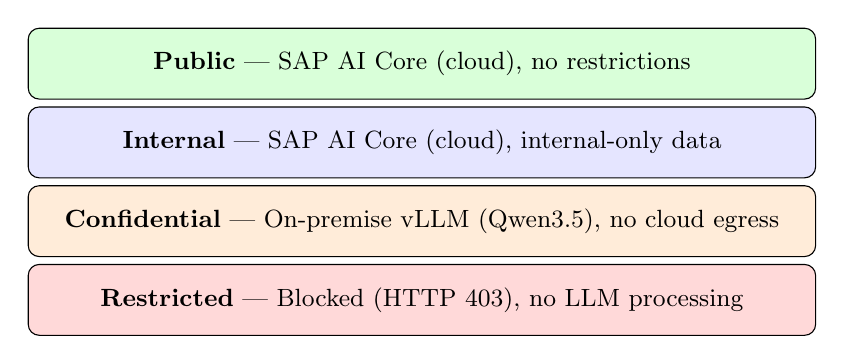
\begin{tikzpicture}[
  tier/.style={rectangle, draw, rounded corners, minimum width=10cm,
               minimum height=0.9cm, font=\small, align=center},
]
  \node[tier, fill=green!15] (t1) at (0,3) {\textbf{Public} --- SAP AI Core (cloud), no restrictions};
  \node[tier, fill=blue!10] (t2) at (0,2) {\textbf{Internal} --- SAP AI Core (cloud), internal-only data};
  \node[tier, fill=orange!15] (t3) at (0,1) {\textbf{Confidential} --- On-premise vLLM (Qwen3.5), no cloud egress};
  \node[tier, fill=red!15] (t4) at (0,0) {\textbf{Restricted} --- Blocked (HTTP 403), no LLM processing};
\end{tikzpicture}
\caption{Four-tier security classification hierarchy}
\label{fig:security-tiers}
\end{figure}

\subsection{On-Premise vLLM for Sensitive Data}

Confidential data is routed to the on-premise vLLM instance running Qwen3.5
models. This ensures that sensitive business data (customer records, financial
data, personal information) never leaves the organization's network perimeter.

The TypeScript router maps three model aliases to their on-premise counterparts
(lines~116--120 of \texttt{intent-router.ts}):

\begin{itemize}
  \item \texttt{qwen3.5-confidential} $\rightarrow$ \texttt{Qwen/Qwen3.5-35B}
  \item \texttt{qwen3.5-0.8b-confidential} $\rightarrow$ \texttt{Qwen/Qwen3.5-0.8B}
  \item \texttt{qwen3.5-9b-confidential} $\rightarrow$ \texttt{Qwen/Qwen3.5-9B}
\end{itemize}

\subsection{Keyword-Based Content Classification}

When no explicit security headers or model hints are provided, the system
falls back to content-based classification. This provides a safety net that
catches sensitive data even when callers omit governance headers.

The keyword system operates at three levels:

\begin{enumerate}
  \item \textbf{Restricted keywords} (\texttt{restricted}, \texttt{classified},
        \texttt{secret}) $\rightarrow$ Block the request entirely.
  \item \textbf{Confidential keywords} (17 terms covering business entities,
        financial data, and personal information) $\rightarrow$ Route to
        on-premise vLLM.
  \item \textbf{PAL keywords} (15 terms covering analytics and ML operations)
        $\rightarrow$ Route to SAP HANA PAL analytics backend.
\end{enumerate}

The keyword lists are canonical and must be kept in sync across three
repositories: \texttt{cap-llm-plugin}, \texttt{ai-core-streaming}, and
\texttt{genui-renderer} (documented at line~124 of \texttt{intent-router.ts}).

\subsection{Component Deny Lists}

The \texttt{SchemaGenerator} enforces a security deny list that prevents the
LLM from generating UI schemas containing potentially dangerous components.
Four components are blocked (lines~22--27 of \texttt{schema-generator.ts}):

\begin{itemize}
  \item \texttt{ui5-file-uploader}: OS file picker enabling potential data
        exfiltration.
  \item \texttt{ui5-file-chooser}: Same risk as file uploader.
  \item \texttt{ui5-upload-collection}: Agent-driven upload flows that could
        bypass data governance.
  \item \texttt{ui5-upload-collection-item}: Child component of upload
        collection.
\end{itemize}

Additionally, the \texttt{sanitizeProps} method (lines~455--473 of
\texttt{schema-generator.ts}) strips all event handler attributes
(\texttt{on*}) and \texttt{javascript:} URLs from component properties,
preventing XSS attacks in LLM-generated UI schemas.

\subsection{Endpoint Safety Validation}

The \texttt{IntentRouter} validates all configured endpoints against a
blocklist of dangerous host prefixes (lines~46--76 of
\texttt{intent-router.ts}):

\begin{lstlisting}[language=TypeScript,caption={Blocked host prefixes (intent-router.ts, lines 46--76)},firstnumber=46]
const BLOCKED_HOST_PREFIXES_IR =
  ['169.254.', '100.100.', 'fd00:', '::1'];

function _irSafeEnvUrl(
    envVar: string, localFallback: string)
    : string {
  // ... URL parsing and validation ...
  for (const prefix of BLOCKED_HOST_PREFIXES_IR) {
    if (host.startsWith(prefix)) {
      console.error(`IntentRouter: ${envVar} `
        + `targets blocked host prefix `
        + `"${prefix}"`);
      return localFallback;
    }
  }
  // ...
}
\end{lstlisting}

This prevents SSRF attacks by rejecting link-local, CGNAT, and unique-local
IPv6 addresses as routing targets.

% ═══════════════════════════════════════════════════════════════════════════════
\section{Cross-Layer Routing Consistency}
\label{sec:consistency}
% ═══════════════════════════════════════════════════════════════════════════════

The TypeScript \texttt{IntentRouter} and Python \texttt{MeshRouter} are
designed as parallel implementations of the same routing logic. Both share:

\begin{enumerate}
  \item The same cascading priority order (forced $\rightarrow$ service
        $\rightarrow$ security $\rightarrow$ model $\rightarrow$ content
        $\rightarrow$ default).
  \item Overlapping service routing maps (7 shared entries).
  \item Identical confidential keyword lists (with minor additions in
        TypeScript for business entities).
  \item The same audit logging structure (\texttt{request\_id},
        \texttt{backend}, \texttt{reason}, \texttt{model}, \texttt{status},
        \texttt{trace\_id}).
\end{enumerate}

There is one notable divergence: the TypeScript router maps
\texttt{restricted} $\rightarrow$ \texttt{blocked} (line~101 of
\texttt{intent-router.ts}), while the Python router maps
\texttt{restricted} $\rightarrow$ \texttt{vllm} (line~34 of
\texttt{router.py}). The TypeScript behavior is the more conservative policy,
as it prevents any LLM processing of restricted data.

\begin{table}[h]
\centering
\caption{Cross-Layer Routing Comparison: TypeScript vs.\ Python}
\begin{tabular}{@{}llll@{}}
\toprule
\textbf{Feature} & \textbf{IntentRouter (TS)} & \textbf{MeshRouter (Py)} & \textbf{Match} \\
\midrule
Backend count & 5 & 2 & TS superset \\
Service map entries & 8 & 7 & TS superset \\
Security classes & 4 & 4 & Yes \\
\texttt{restricted} target & \texttt{blocked} & \texttt{vllm} & Divergent \\
Model aliases & Qwen3.5 family & GPT/Claude & Different focus \\
Content keywords & 17 + 3 + 15 & 9 & TS superset \\
Audit log & Via OTel spans & In-memory list & Different mechanism \\
\bottomrule
\end{tabular}
\end{table}

% ═══════════════════════════════════════════════════════════════════════════════
\section{Conclusion}
\label{sec:conclusion}
% ═══════════════════════════════════════════════════════════════════════════════

The prompt-to-response routing system implements a multi-layer classification
architecture that enforces data governance, security classification, and
intelligent backend selection at every level of the request pipeline. The
cascading decision tree ensures that explicit governance signals (forced
headers, service policies, security classifications) always take precedence
over implicit content analysis, while the keyword-based fallback provides a
safety net for unclassified requests.

Key design properties of the system:

\begin{itemize}
  \item \textbf{Defense in depth}: Seven classification levels ensure no
        request reaches a backend without explicit or implicit authorization.
  \item \textbf{Data sovereignty}: Confidential data is guaranteed to remain
        on-premise via vLLM routing, with no cloud egress.
  \item \textbf{Auditability}: Every routing decision is logged with
        structured metadata (request ID, backend, reason, model, trace ID)
        for compliance and debugging.
  \item \textbf{UI security}: The schema generator's deny list and prop
        sanitization prevent LLM-generated UI from introducing XSS or data
        exfiltration vectors.
  \item \textbf{Contract enforcement}: The CDS service definition provides a
        typed API contract that drives code generation and drift detection.
  \item \textbf{Streaming support}: End-to-end SSE streaming with structured
        frame protocols (delta/done/error) enables real-time token delivery.
\end{itemize}

\end{document}
